\documentclass[11pt]{article}
\usepackage[margin=1in]{geometry}
\usepackage{graphicx} % Required for inserting images
\usepackage{float}
\usepackage{natbib}

\title{Lab 1-PECARN TBI Data,Stat 214, Spring 2026}
\date{February 2026}

\begin{document}

\maketitle

\section{Introduction}
Traumatic brain injury in children is a common reason for emergency department visits and frequently leads to CT imaging. While CT scans are valuable for detecting clinically important traumatic brain injuries (ciTBI), they expose children to radiation, which carries long-term malignancy risk. Identifying children at very low risk of ciTBI is therefore essential to reduce unnecessary imaging without compromising safety.\\
This exploratory data analysis (EDA) examines a large prospective pediatric TBI dataset derived from the PECARN study (\cite{kuppermann2009identification}). The purpose of this analysis is to understand the structure, quality, and clinical relationships within the data, identify inconsistencies or missingness patterns, and prepare the dataset for meaningful modeling and interpretation. By better understanding symptom patterns, injury mechanisms, and clinical findings associated with ciTBI, we can gain insight into how data quality affects clinical prediction. 
Please Note: A notebook is added in the code section to reproduce every step taken.

\section{Data}
The dataset consists of pediatric patients younger than 18 years presenting within 24 hours of head trauma. It includes demographic information, examination findings, reported symptoms, injury mechanisms, imaging information, and important outcomes.
The primary outcome of interest is clinically important traumatic brain injury (ciTBI), defined according to the original study criteria. Predictor variables include mental status indicators, loss of consciousness, vomiting, skull fracture signs, and injury mechanism severity. These variables directly relate to the domain problem: identifying children at low risk for ciTBI in order to safely reduce CT scans.
\section{Data Collection}
The data was collected as part of a large prospective cohort study conducted across multiple emergency departments in North America. Physicians completed standardized forms at the time of clinical evaluation, documenting symptoms, examination findings, and injury characteristics prior to imaging results being known.
Most variables are categorical (e.g., Yes/No/Unclear, duration categories, or not applicable codes).Some variables are hierarchical (e.g., vomiting timing recorded only if vomiting occurred), and others depend on age (e.g., fontanelle bulging in infants). 
\section{Data Cleaning}
    \subsection{Initial Structure Inspection}
    As a first step, an initial exploration of the dataset was conducted to understand the data. The overall shape (number of rows and columns) was examined and confirmed to match the \cite{kuppermann2009identification}. \\    
    \subsection{Verification of Key Identifier}
    Checks were performed to identify: missing Patient Numbers and duplicate Patient Numbers; no such instances were found.
    \subsection{Inclusion-Exclusion Criteria}
    \textbf{Age Consistency}\\
    All observations satisfied the age requirement(less than 18). Additionally, the age recorded in months was consistent with the age recorded in years.\\
    \textbf{GCS Score}\\
    Patients with a score lower than 14 were identified, instead of dropping these a different dataframe was created to analyse these patients separately. These cases may provide valuable insights and therefore were not excluded from the dataset.
    \subsection{Outcome Column: PosIntFinal}
    While checking the PosIntFinal column containing the main outcome,18 observations were found to have missing outcome values.
    Upon exploring more, these patients were:
    \begin{itemize}
    \item Transferred to general admission
    \item Kept for less than 24hours 
    \item Transferred to other hospitals
    \end{itemize}
    Since, these patients were not followed up, such inconclusive data cannot be included in the study. Therefore, these 18 rows are dropped.
    \subsection{Injury Mechanism and Injury Severity Consistency}
    The relationship between InjuryMechanism and High\_impact\_InjSev was examined for consistency.Two inconsistencies were identified:
    \begin{itemize}
    \item Thirty-three observations contained valid InjuryMechanism values but had missing values in High\_impact\_InjSev.
    \item Three hundred one observations had both injury mechanism and injury severity missing.
    \end{itemize}
    To address the first inconsistency, High\_impact\_InjSev values were updated according to the corresponding InjuryMech values.
    For the second issue, on further exploration, there seems to be a relation with high severity cases. In cases which have eventually led to ciTBI were correlated with missing Injury Mechanism and Injury Severity columns.
    \begin{figure}[H]
        \centering
        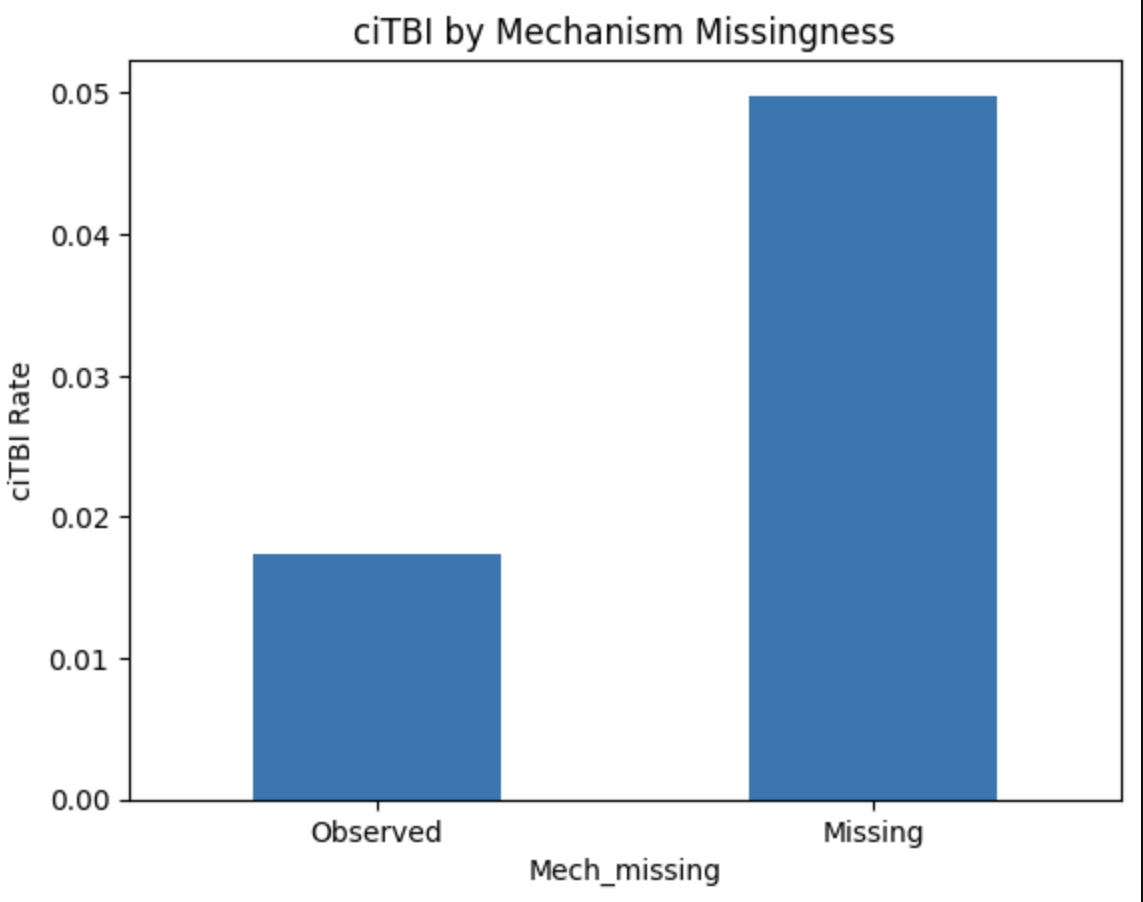
\includegraphics[width=0.5\linewidth]{Screenshot 2026-02-18 at 7.25.56 PM.png}
        \caption{ciTBI rate vs Injury Mechanism missigness}
        \label{fig:placeholder}
    \end{figure}
    Imputing such rows with estimated values might change the meaning of the data, thus a new category is created for this case. For InjuryMech: 99(signifying "Missing") and for High\_impact\_InjSev: 4(signifying "Mechanism not documented")
    \subsection{Loss of Consciousness and Seizure Variables}
    Variables LOCSeparate and LocLen have a huge number of missing values. Scenarios that were encountered and how it was addressed:
    \begin{itemize}
        \item The LOCSeparate variable was examined and found to contain missing values. On further inspection, analysis inidicated that there is a 6.7\% rate of ciTBI in patients with missing LOCSeparate values. Also, they are more likely to be sedated, intubated and less likely to act normally.Therefore, a new category was created: 3( Unknown/Missing) to preserve information.
        \begin{figure}[H]
            \centering
            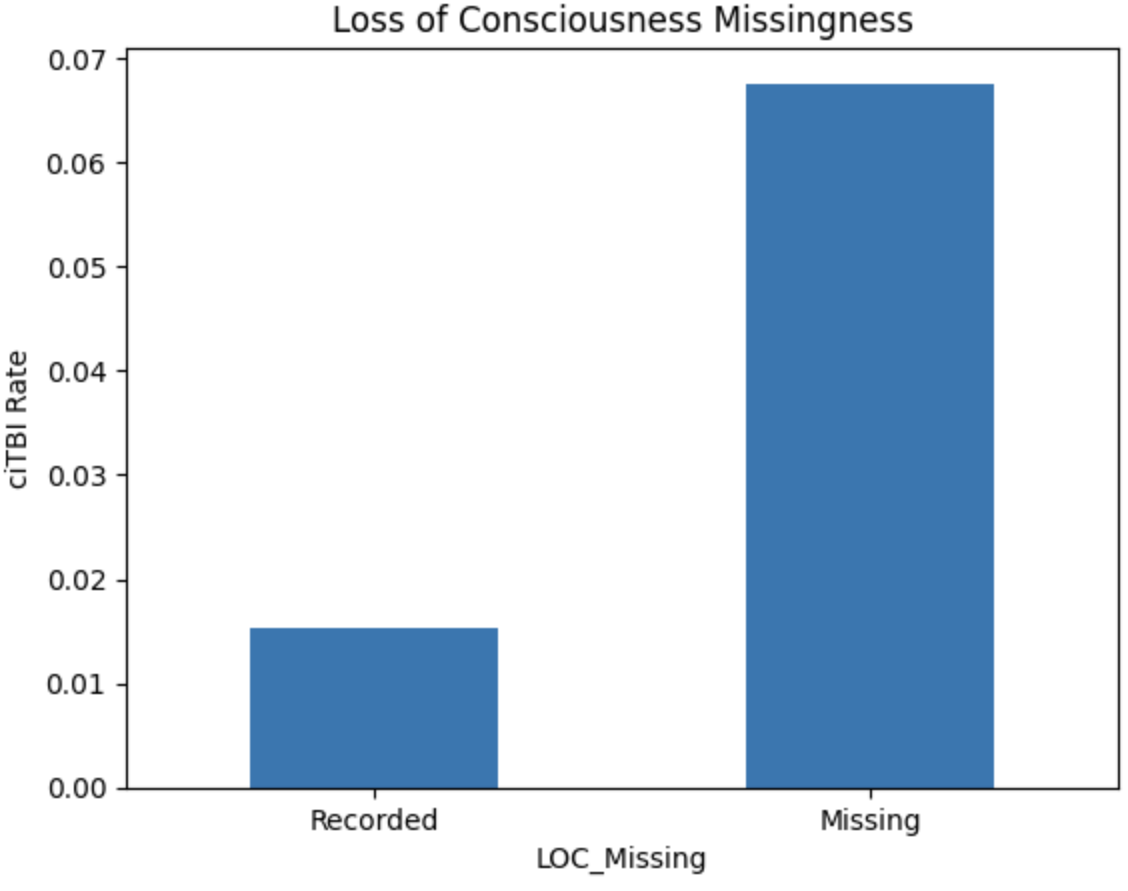
\includegraphics[width=0.5\linewidth]{Screenshot 2026-02-18 at 11.51.05 PM.png}
            \label{fig:placeholder}
        \end{figure}
        \begin{figure}[H]
            \centering
            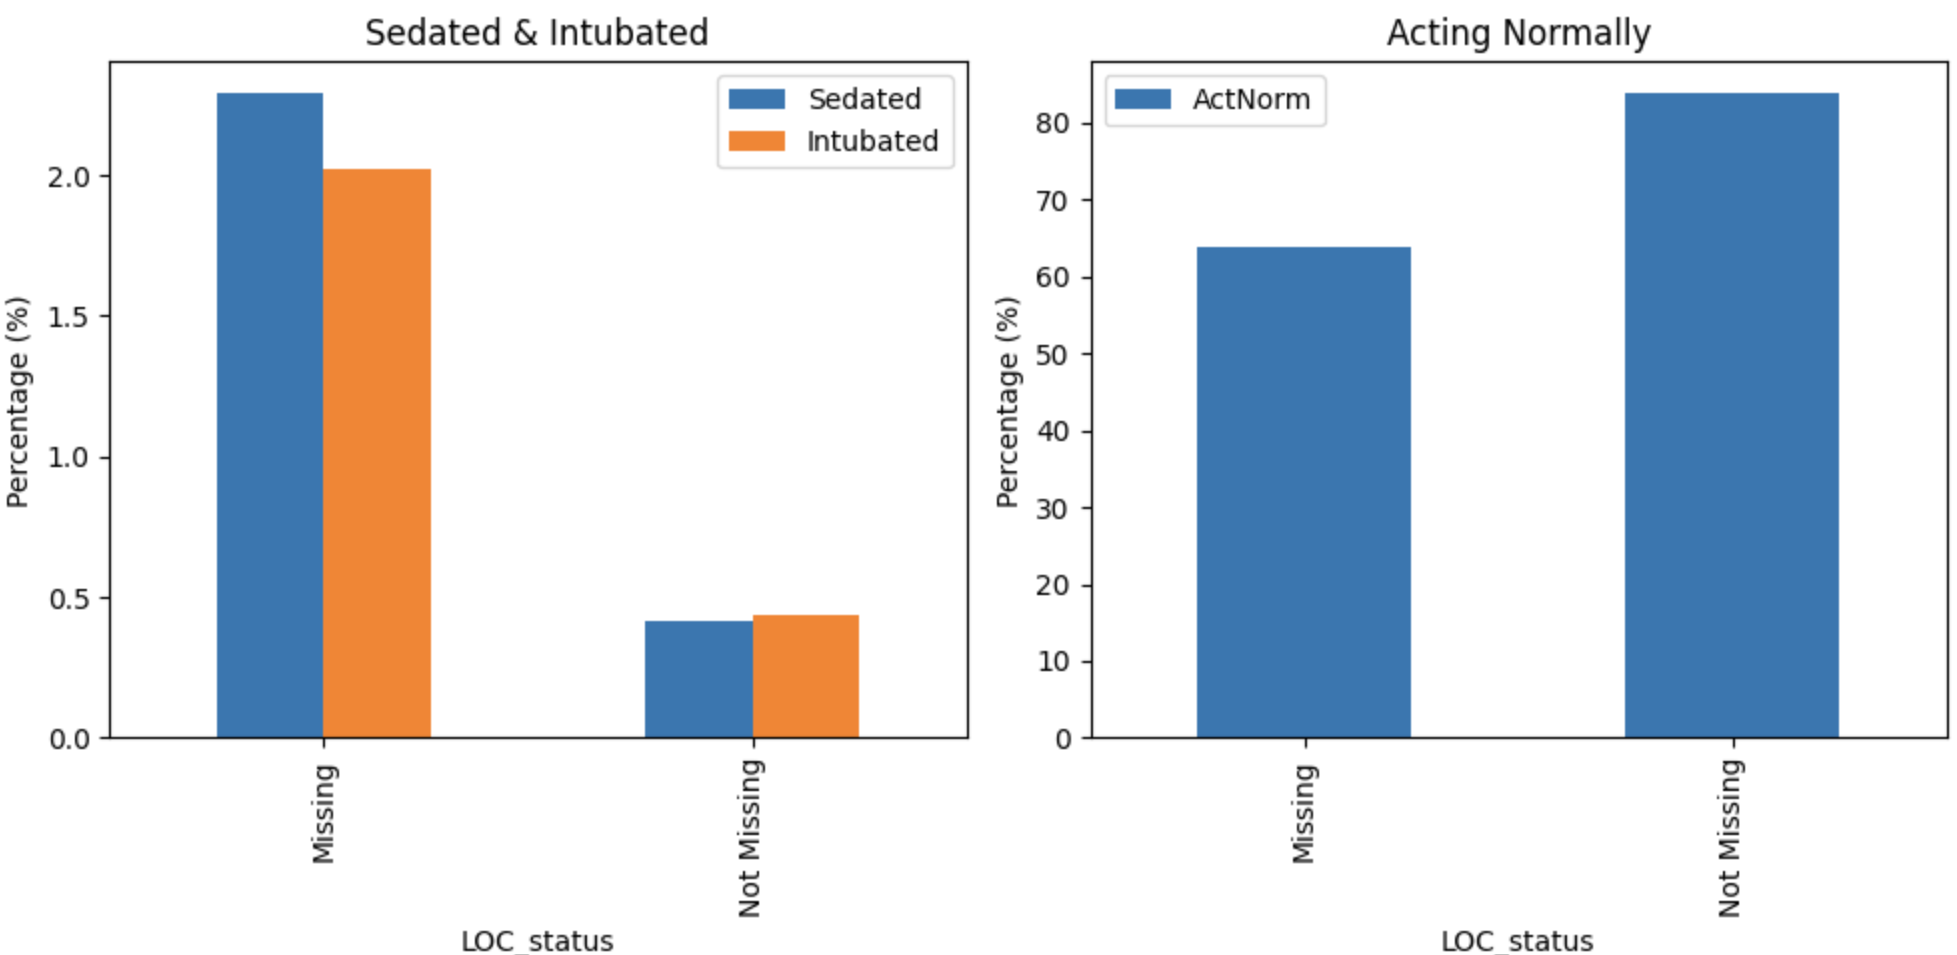
\includegraphics[width=0.75\linewidth]{Screenshot 2026-02-19 at 12.20.51 AM.png}
            \label{fig:placeholder}
        \end{figure}
        \item LocLen null values: On inspection, it can be concluded that this column has null values for when LOCSeparate is a "Yes" or "Suspected" but for some reasons, the length of LOC was not recorded. For such scenarios, a new category(5: Missing/Unknown length) is created.
    \end{itemize}
    A similar pattern is discovered with the Seizure related data(Seiz, SeizOccur and SeizLen). Similar to above a new category(2- undocumented) is created for the \textbf{Seiz} column. Since, occurrence of seizure is rare, with instances of Seizure, imputing the SeizOccur and SeizLen columns to have the mean values would remove the variability. Thus, a new category was created. SeizOccur: 4(undocumented) and SeizLen: 5(undocumented).
    \subsection{Amnesia, Headache and Dizziness}
    Over a 1000 rows were found to have null values or data recorded for these columns for age less than 2 years. These rows were corrected to store 91(Pre-verbal/Non-verbal) category.
    Amnesia, Headache and Dizziness columns were found to have missing values for instances where patient was paralyzed, sedated, intubated, not acting normal or had altered mental state. For such cases, a category was created to denote the severity.
    Rest of the rows with unexplainable null values were marked as "Undocumented". \\
    Certain rows were null under columns for severity of headache and start of headache. These were updated to 92 where HA\_verb has a value 91 and for the rest were marked with a new category denoting "Undocumented".
    \subsection{Altered Mental State}
    Missing values were found in cases where GCS total = 15. These were updated to be 0 as the definition set for AMS was that GCS Score had to be less than 15.
    \subsection{Acting Normal as per Parent}
    Approximately 7\% of values were missing. Because missingness was associated with a higher ciTBI rate, missing values were not recoded as “normal.” Instead, a separate “Unknown” category was created to preserve potential clinical signal and avoid bias.
    \subsection{Vomit and Related Variables (VomitNbr, VomitStart, VomitLast)}
    \begin{itemize}
        \item Missing primary vomiting status (Vomit) was updated as a new “Undocumented” category.
        \item When Vomit = 0 (no vomiting), related detail variables were set to “Not applicable” (92).
        \item When Vomit = 1 but episode number or timing variables were missing, new “Undocumented” categories were created rather than imputing values.
    \end{itemize}
    This preserved the clinical structure of the variable and avoided speculative imputation.
    \subsection{SFxPalp (Palpable Skull Fracture) and SFxPalpDepress}
    \begin{itemize}
        \item Missing SFxPalp values were recoded as “Undocumented”, consistent with the study documentation and prediction rule.
        \item SFxPalpDepress: if no palpable fracture was present, it was coded as “Not applicable.”
    \end{itemize}
    \subsection{FontBulg (Anterior Fontanelle Bulging)}
    Since fontanelle bulging is clinically relevant primarily in infants:For children older than 2 years, missing values were coded as “No”. For age less than 2 years with missing values, a separate “Undocumented” category was created.
    \subsection{Variables Determining PosIntFinal}
    The outcome variable \textbf{PosIntFinal} is determined by the variables \textbf{DeathTBI, HospHead, HospHeadPosCT, Intub24Head,} and \textbf{Neurosurgery}. Missing values in these columns were imputed based on the recorded outcome. For cases with a non-ciTBI outcome (PosIntFinal = 0), missing values were replaced with 0. For \textbf{Intub24Head}, missing values were set to 1 when the outcome was positive (ciTBI) and 0 otherwise. The \textbf{HospHeadPosCT} column contained no missing values.
    
\section{Data Exploration}
We begin by examining the distribution of key variables, particularly age, to understand the population composition.Next, we explore the major clinical predictors, including altered mental status (AMS), vomiting, loss of consciousness, mechanism of injury, and skull fracture findings.\\
We also examine the overall rate of ciTBI and CT utilization to contextualize the dataset within clinical practice. Comparing outcome rates across key predictors allows us to assess which clinical features are most strongly associated with ciTBI. These exploratory comparisons motivate the selection of variables for deeper analysis and support the clinical logic underlying prediction rules.\\
Finally, we evaluate patterns of missingness across core predictors. By identifying whether missing values occur more in severe cases, we assess potential sources of bias and justify the data cleaning decisions described earlier.
\section{Findings}
    \subsection{Low-risk children still received CT imaging, often driven by subjective or provider factors}
    Among patients classified as low-risk by injury severity and absence of head trauma, CT scans were still commonly performed. Imaging decisions appear strongly associated with symptoms such as vomiting, loss of consciousness, headache, and amnesia rather than injury severity alone. This suggests potential over utilization of CT in clinically low-risk populations and highlights variability between clinical decision making and validated risk stratification rules.
    \begin{figure}[H]
        \centering
        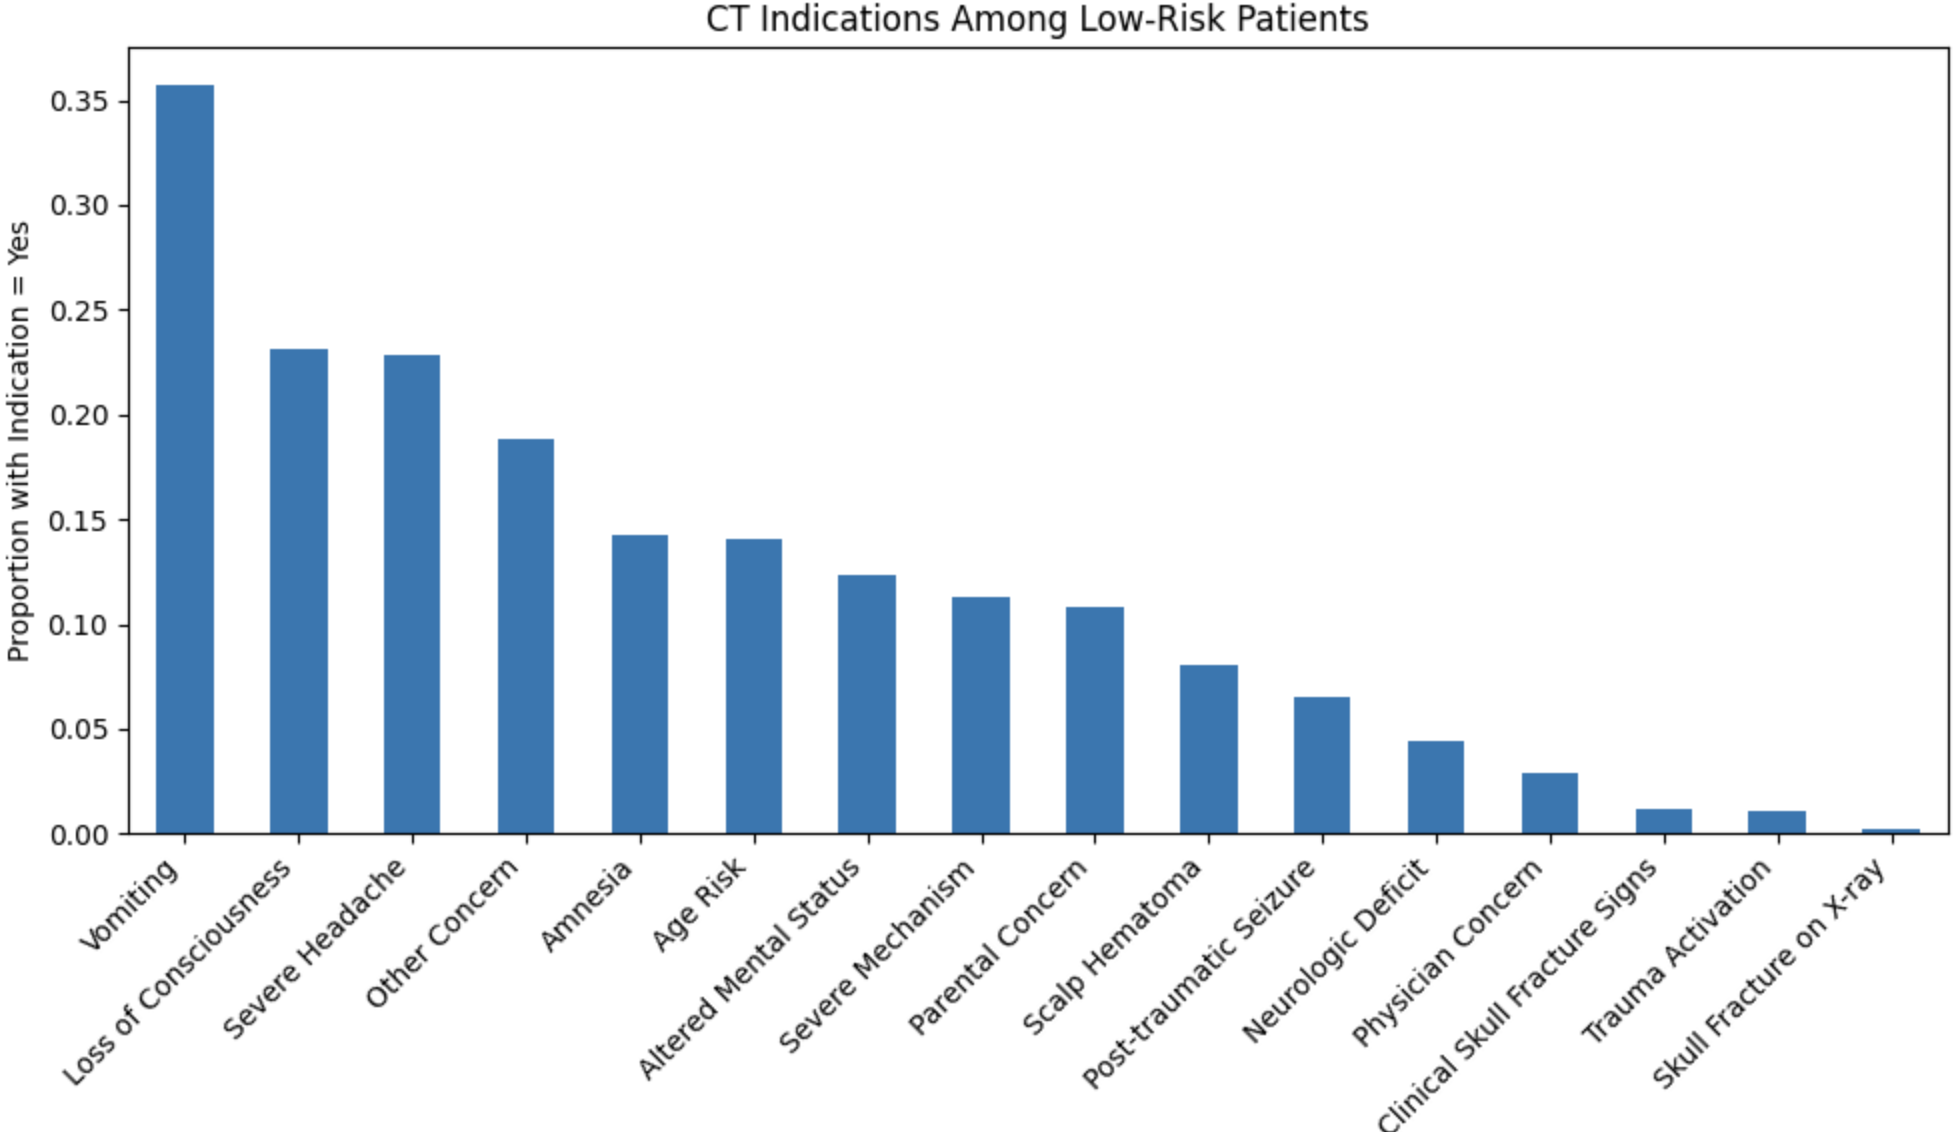
\includegraphics[width=1 \linewidth]{Screenshot 2026-02-20 at 1.15.47 AM.png}
        \caption{Distribution of CT indication variables among patients classified as low injury severity and without head trauma. Subjective or provider-driven indications contributed substantially to imaging decisions.}
        \label{fig:placeholder}
    \end{figure}
    \subsection{Missing Clinical Assessments Are Associated With Higher ciTBI Rates}
    We observed that patients with missing documentation for key clinical variables such as “Acting normally as per parent” (ActNorm); this variable had substantially higher rates of clinically important traumatic brain injury (ciTBI) compared to those with documented assessments. Specifically, the ciTBI rate among patients with missing ActNorm values was markedly higher than among those with recorded responses.\\
    This suggests that missingness in certain clinical fields is not random but may reflect greater clinical severity, incomplete assessment in urgent situations, or documentation gaps in higher-risk cases. Therefore, treating missing values as a separate category preserves meaningful clinical signal and avoids biasing results by incorrectly assuming normal findings.
    \begin{figure}[H]
        \centering
        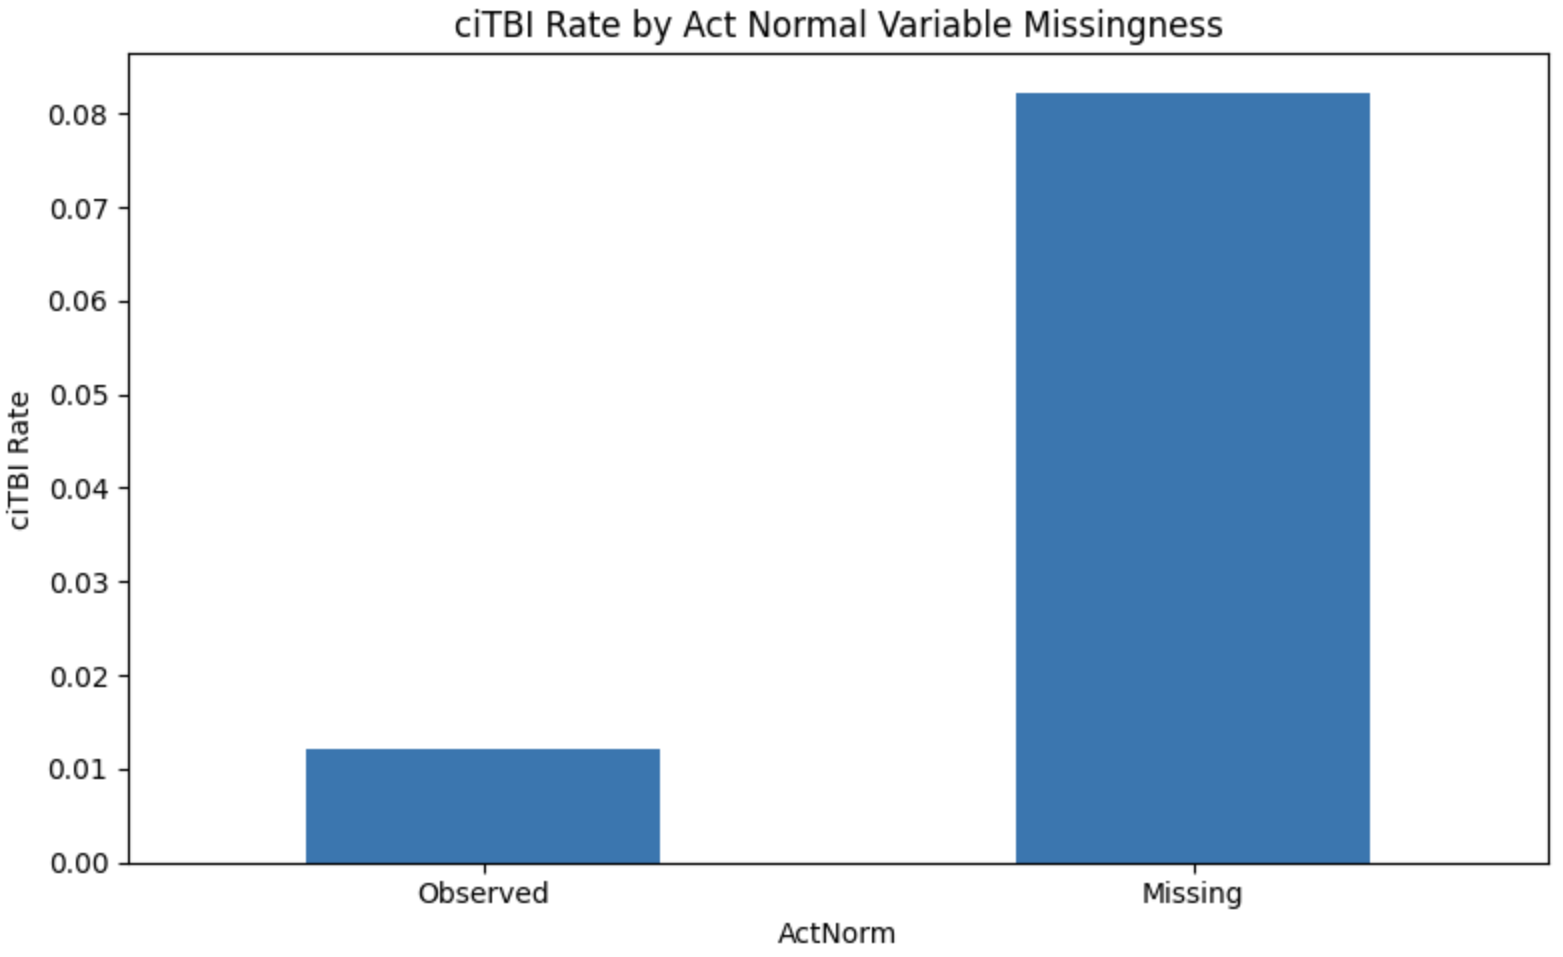
\includegraphics[width=0.75\linewidth]{Screenshot 2026-02-20 at 1.21.23 AM.png}
        \caption{Patients with missing documentation of “acting normally” had substantially higher ciTBI rates, suggesting non-random missingness related to clinical severity.}
        \label{fig:placeholder}
    \end{figure}
    \subsection{Severe Mechanism Strongly Increases ciTBI Risk}
    The ciTBI rate increases substantially with greater injury mechanism severity. Patients classified as having low-severity mechanisms had the lowest ciTBI rates, while moderate and high-severity mechanisms were associated with progressively higher risk. Notably, patients with undocumented mechanism severity demonstrated ciTBI rates comparable to or higher than the high-severity group, suggesting that missing documentation may reflect more clinically complex or severe presentations.\\
    This finding reinforces the importance of injury mechanism as a core predictor in risk stratification. It also highlights that undocumented or unclear mechanism data should not be assumed to represent low risk, as these cases may carry elevated clinical concern.
    \begin{figure}[H]
        \centering
        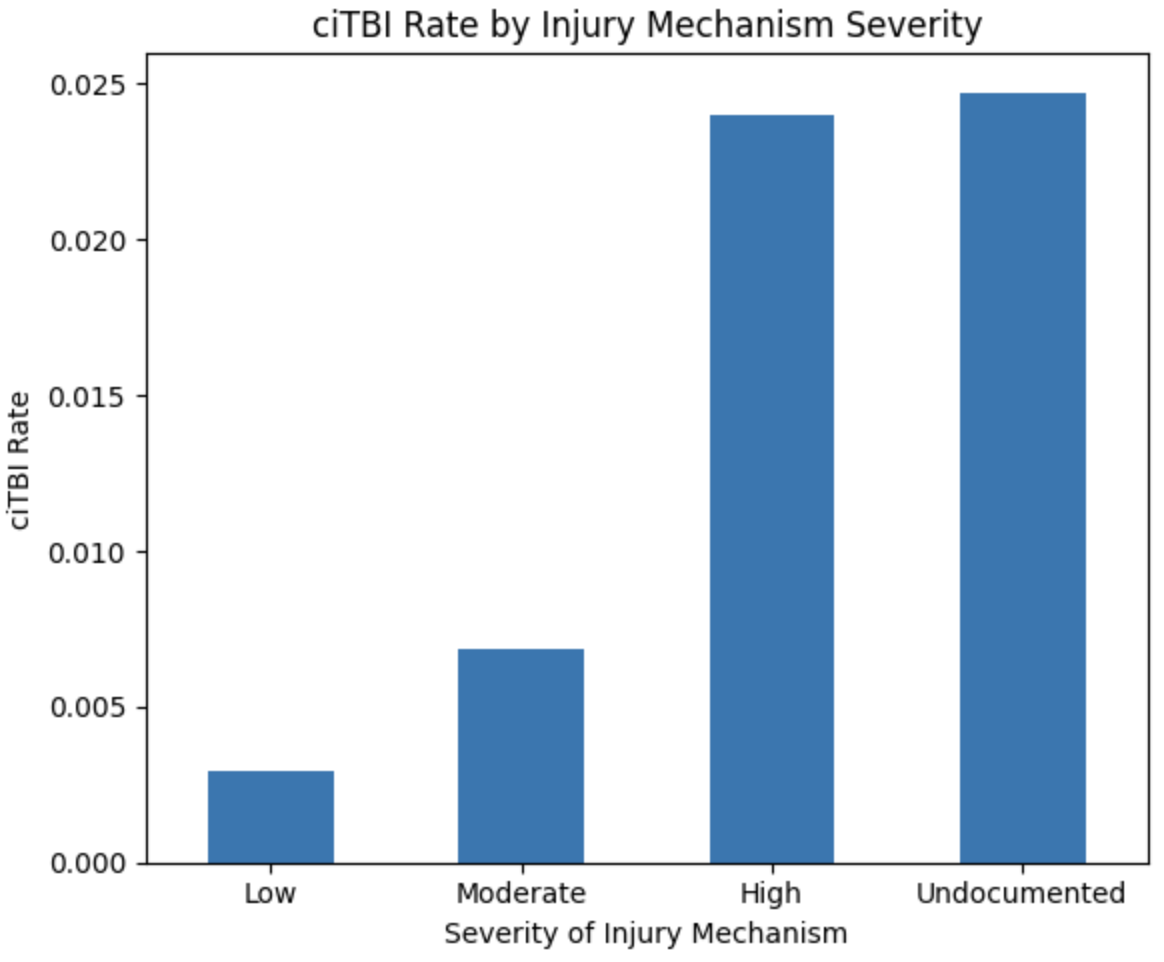
\includegraphics[width=0.75\linewidth]{Screenshot 2026-02-20 at 1.29.19 AM.png}
        \caption{ciTBI rates increase substantially with injury mechanism severity, supporting its importance as a core risk predictor}
        \label{fig:placeholder}
    \end{figure}
\section{Reality Check}
To validate the cleaned dataset, we examined the overall ciTBI rate (~0.9\% in the original publication), the proportion of CT utilization, and the increasing trend in ciTBI risk across injury mechanism severity categories.\\
Our assumption is that, after cleaning, the dataset should preserve the fundamental clinical relationships described in the published study. This comparison is useful because it ensures that cleaning decisions did not distort clinically established patterns.\\
The cleaned dataset passes this reality check. The overall ciTBI rate remains low and comparable to published values, and the expected monotonic increase in risk across mechanism severity categories is preserved.
\begin{figure}[H]
    \centering
    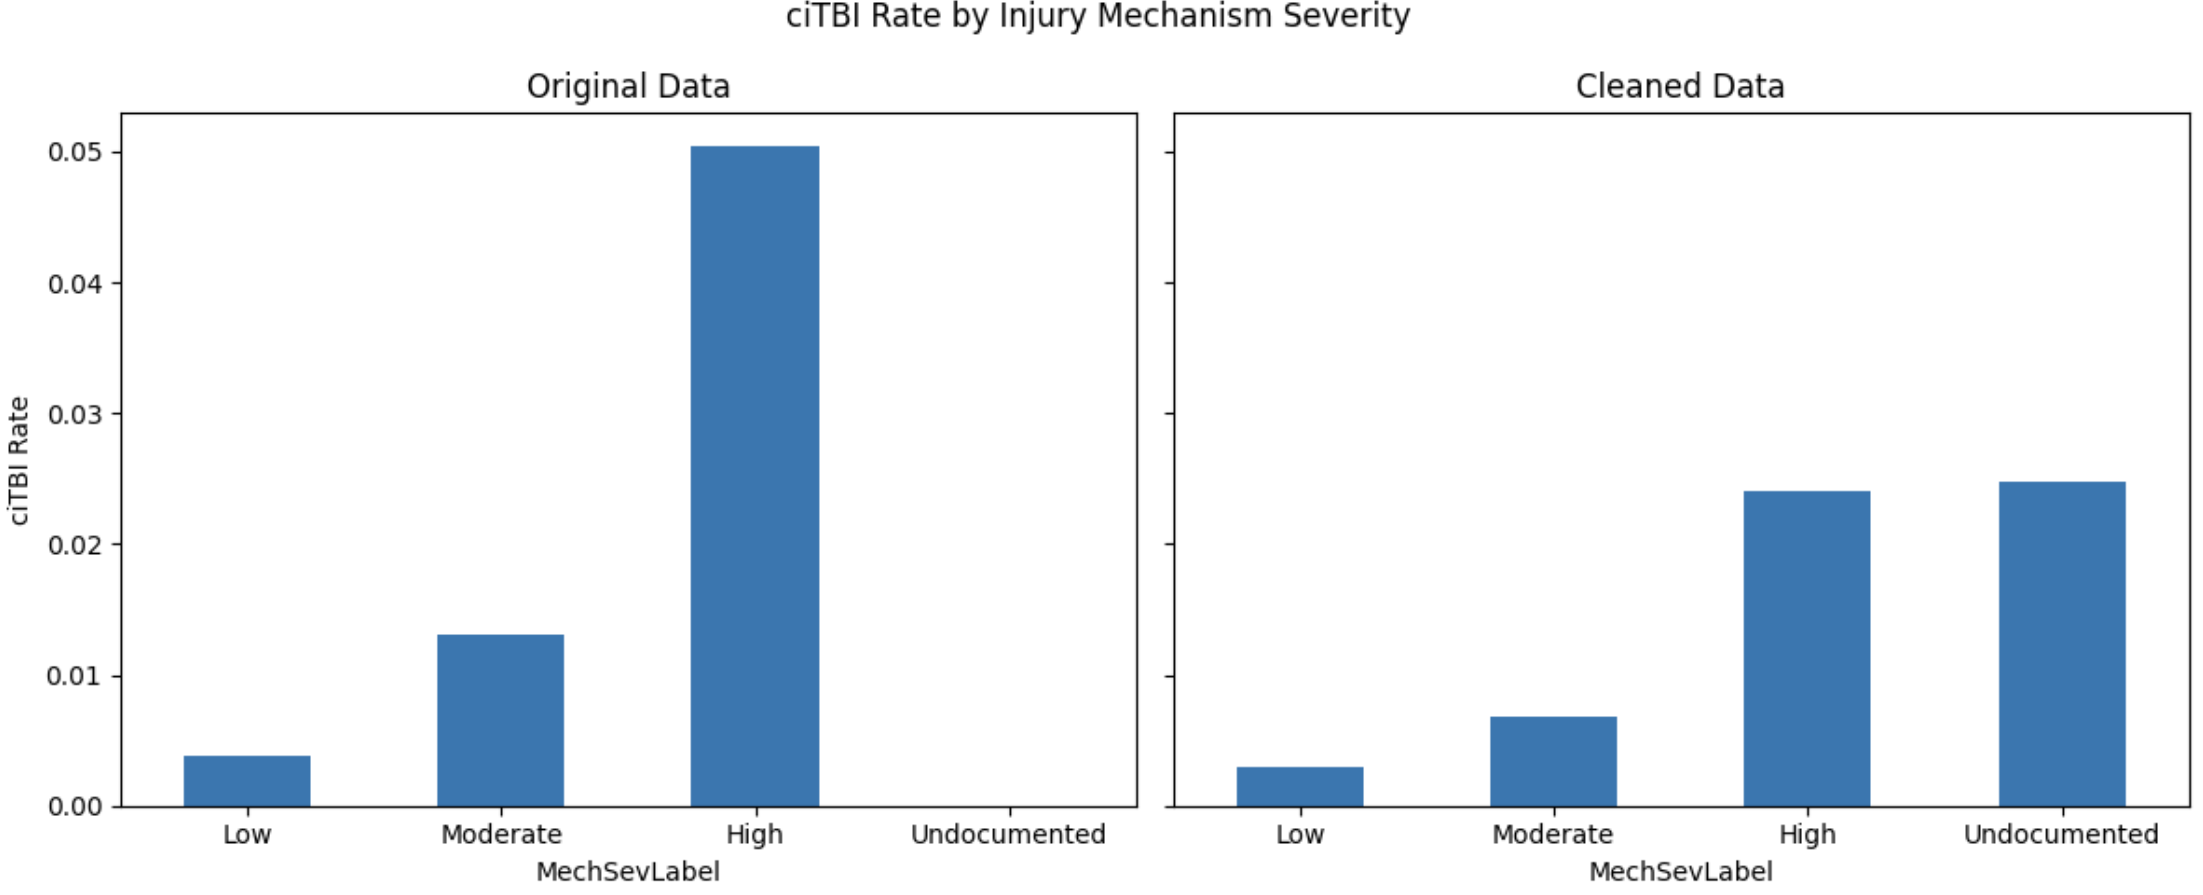
\includegraphics[width=1 \linewidth]{Screenshot 2026-02-20 at 11.53.41 AM.png}
    \label{fig:placeholder}
\end{figure}
\section{Stability}
To assess robustness, we re-examined Finding 3 (ciTBI rate by injury mechanism severity) after perturbing the data by reclassifying “Undocumented” mechanism severity as “Low” severity. This tests whether the observed risk gradient is sensitive to how missing mechanism data are handled.The before and after comparison showed that although absolute rates shifted slightly, the overall increasing trend from low to high severity persisted.This stability check suggests that the association between injury mechanism severity and ciTBI risk is robust and not driven solely by cleaning choices.
\begin{figure}[H]
    \centering
    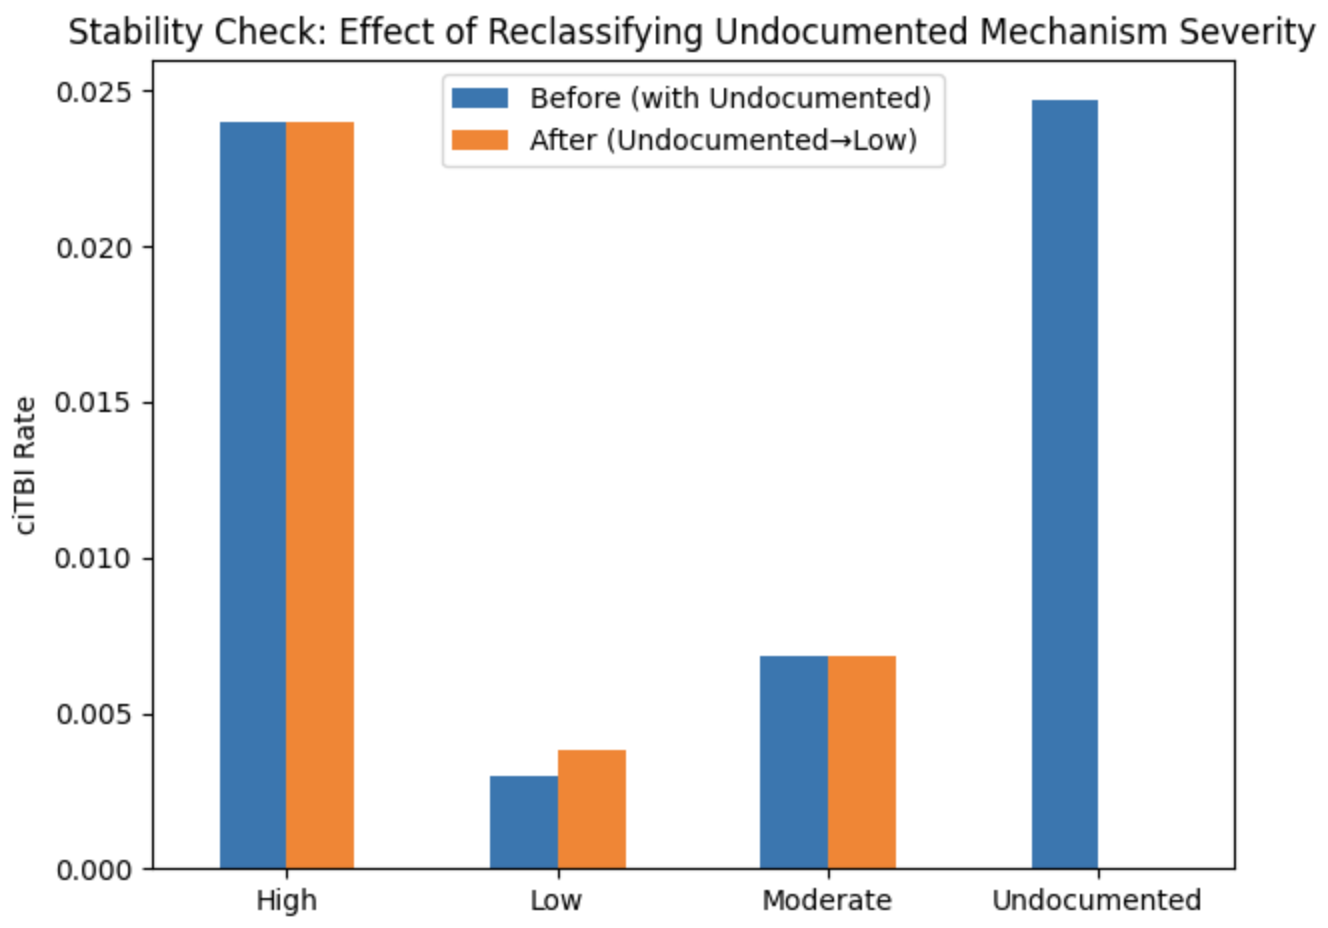
\includegraphics[width=0.75\linewidth]{image.png}
    \label{fig:placeholder}
\end{figure}
\section{Modeling}
    \subsection{Implementation}
    \textbf{Modeling Design Choices}:
    We implemented three classification approaches to predict whether a CT scan should be recommended:
    \begin{itemize}
        \item PECARN-style Clinical Decision Rule (CDR): A rule-based implementation based on \cite{kuppermann2009identification}. This model uses predefined clinical criteria without parameter tuning. It serves as a transparent benchmark aligned with clinical practice.
        \item Logistic Regression: A linear probabilistic model trained using cleaned predictor variables. Default L2 regularization was used and decision threshold was set to 0.5.
        Performance evaluated using accuracy, precision, recall, AUC(area under curve), and confusion matrix.
        \item Random Forest: A non-linear ensemble model to capture complex feature interactions.Default sklearn hyperparameters were used (number of trees, depth not aggressively tuned to avoid overfitting) and decision threshold = 0.5. It was evaluated using the same metrics as logistic regression.
    \end{itemize}
    All models were trained on the same cleaned dataset with a consistent train–test split to ensure fair comparison.
    
    \begin{table}[ht]
    \centering
    \caption{Model Performance Comparison}
    \begin{tabular}{lcccccccc}
    \hline
    Model & Accuracy & Precision & Recall & AUC \\
    \hline
    PECARN Rule & 0.7567 & 0.6240 & 0.7818 & --  \\
    Logistic Regression (0.5) & 0.7795 & 0.7642 & 0.5426 & 0.8279 \\
    Random Forest (0.5) & 0.8128 & 0.7835 & 0.6489 & 0.8668 \\
    \hline
    \end{tabular}
    \label{tab:model_comparison}
    \end{table}
    The PECARN rule achieves the highest recall (0.782), reflecting strong sensitivity and a lower likelihood of missing ciTBI cases, but at the cost of lower precision and more false positives. Logistic regression improves precision (0.764) and overall accuracy (0.780) but substantially reduces recall, indicating more missed cases. The random forest model provides the best overall performance, with the highest accuracy (0.813) and AUC (0.867), and offers a more balanced trade-off between precision and recall. These results suggest that while PECARN prioritizes sensitivity for clinical safety, the machine learning models—particularly random forest—demonstrate superior overall predictive performance.
    \begin{figure}[H]
        \centering
        
\includegraphics[width=0.75\linewidth]{model_accuracy.png}
        \caption{Model Accuracy}
        \label{fig:placeholder}
    \end{figure}
    \subsection{Interpretability}
    \begin{itemize}
        \item CDR - PECARN: It is highly interpretable and has transparent clinical logic. It is also easy to explain to medical staff. This rule prioritizes sensitivity.
        \item Logistic Regression: This model is moderately interpretable. The coefficients directly indicate direction and strength of association. This balances interpretability and predictive ability.
        \item Random Forest: It is not inherently interpretable. It achieves the strongest overall discrimination but sacrifices interpretability.
    \end{itemize}
    \begin{figure}[H]
        \centering
        
\includegraphics[width=0.75\linewidth]{rf_feature_importance.png}
        \caption{How to interpret complex models? Example: Random Forest}
        \label{fig:placeholder}
    \end{figure}
\section{Stability}
We perturbed the test data by reclassifying undocumented injury mechanism severity as low severity. Below is the result of modeling when we reclassified the data. If we compare with Table 1 under in Section 9.1, we can see that there is little or almost no change in the results. Thus we can conclude that model's results are stable.
\begin{table}[ht]
    \centering
    \caption{Model Performance Comparison}
    \begin{tabular}{lcccccccc}
    \hline
    Model & Accuracy & Precision & Recall & AUC \\
    \hline
    PECARN Rule & 0.7567 & 0.6240 & 0.7818 & --  \\
    Logistic Regression (0.5) & 0.7789 & 0.7590 & 0.5475 & 0.8281 \\
    Random Forest (0.5) & 0.8106 & 0.7906 & 0.6304 & 0.8670 \\
    \hline
    \end{tabular}
    \label{tab:model_comparison}
    \end{table}
\section{Discussion}
The dataset was quite large and it made sensitivity and false negatives more critical than overall accuracy. Several variables required careful cleaning due to missingness and documentation inconsistencies, and reasonable recoding assumptions (e.g., undocumented mechanism severity) slightly affected results but did not materially change conclusions. The lab spans three realms: the data/reality layer (clinical documentation and measurement), the algorithm/model layer (implementation of decision rules and statistical models), and the future data/reality layer (generalization to new clinical settings). There is no perfect one-to-one mapping between data and reality—clinical variables simplify complex bedside assessments, and visualizations further aggregate this complexity, so model conclusions should be interpreted within these limitations.
\section{Conclusion}
This analysis demonstrates how structured clinical variables from the PECARN dataset can be used to support CT decision-making in pediatric head trauma. The clinical decision rule prioritized sensitivity, while logistic regression and random forest improved discrimination (AUC) and precision, illustrating trade-offs between interpretability and predictive performance. Data cleaning decisions and reasonable perturbations did not substantially alter the main findings, suggesting stability of results. Overall, the study highlights how careful pre-processing, transparent modeling, and validation are essential when translating clinical data into decision-support tools.
\section{Academic Honesty}
To Professor Bin Yu,\\
I certify that this project is my own work. I have cited properly all sources and ideas that are not my own.
\section{Collaborators}
No collaborations done for this project.
\section{Bibliography}
\bibliographystyle{apalike}
\bibliography{ref}
\end{document}
